\documentclass[a4page]{article}
\usepackage[14pt]{extsizes}
\usepackage[utf8]{inputenc}
\usepackage[utf8]{inputenc}
\usepackage[russian]{babel}
\usepackage{amsmath}
\usepackage[left=20mm, top=15mm, right=15mm, bottom=30mm, footskip=15mm]{geometry}
\usepackage{indentfirst}
\usepackage{paralist}

\usepackage{fancyvrb}
\usepackage{framed}
\usepackage{url}
\usepackage{csquotes}

\usepackage{graphicx}
\usepackage{svg}
\graphicspath{ {./images/} }

\usepackage{float}
\floatstyle{ruled}

\usepackage[
	backend=biber,
	sorting=nyt,
	bibstyle=gost-numeric,
	citestyle=gost-numeric
]{biblatex}

\usepackage[
	bookmarks=true, colorlinks=true, unicode=true,
	urlcolor=black,linkcolor=black, anchorcolor=black,
	citecolor=black, menucolor=black, filecolor=black,
]{hyperref}

\addbibresource{sources.bib}

\renewcommand{\baselinestretch}{1.35}

\begin{document}


\begin{titlepage}

	\begin{center}
		\hfill \break
		\textbf{
			\large{РОССИЙСКИЙ УНИВЕРСИТЕТ ДРУЖБЫ НАРОДОВ}\\
			\normalsize{Факультет физико-математических и естественных наук}\\
			\normalsize{Кафедра прикладной информатики и теории вероятностей}\\
		}
		\vspace*{\fill}
		\Large{\textbf{ДОКЛАД\\ на тему <<Оркестрация контейнеров промышленного уровня на базе Kubernetes>>}}
		\\
		\underline{\textit{\normalsize{Дисциплина: Администрирование сетевых подсистем}}}
		\vspace*{\fill}

	\end{center}

	\begin{flushright}
		Студент: \underline{Матюхин Григорий}\\ \vspace{0.5cm}
		Группа: \underline{НПИбд-01-21}
	\end{flushright}


	\begin{center} \textbf{МОСКВА} \\ 2023 г. \end{center}
	\thispagestyle{empty} % выключаем отображение номера для этой страницы

\end{titlepage}

\newpage

\tableofcontents

\newpage
\section{Введение}
Kubernetes (K8s) --- это программная платформа для автоматического управления контейнеризованными приложениями. Она предлагает базовые механизмы для их развертывания, масштабирования и поддержки.

Исходный код системы был представлен в 2014 году. После выхода версии 1.0 в 2015 году Google в сотрудничестве с Linux Foundation основала фонд Cloud Native Computing Foundation (CNCF) и передала ему Kubernetes в рамках начального технологического вклада. Kubernetes сочетает в себе более чем 15-летний опыт Google в масштабировании производственных рабочих нагрузок с лучшими в своем классе идеями и практиками сообщества.

В большинстве компаний инфраструктура построена на Kubernetes --- от маленьких проектов до огромных кластеров и облаков, которые обеспечивают бесперебойную доступность сервисов.

Так что же такое Kubernetes и для чего мы в хотим использовать именно его, а не обычные контейнеры, например Docker.

\section{Методы развертывания}

\includesvg[width=450pt]{./images/Container_Evolution.svg}

\subsection{Традиционное}
Раньше организации запускали приложения прямо на физических серверах. На которых, однако, не было возможности определить границы ресурсов, и это вызывало проблемы с их распределением. Например, если на физическом сервере работает несколько приложений, могут быть случаи, когда одно приложение будет занимать большую часть ресурсов, и в результате другие приложения будут работать хуже. Решением этой проблемы было бы запуск каждого приложения на отдельном физическом сервере. Но это масштабируется плохо, поскольку одно приложение не использует все доступные ресурсы одного сервера, и содержать множество таких серверов дорого.

\subsection{Виртуализированное}
Решением этой проблемы была виртуализация. Она позволяет запускать несколько виртуальных машин на одном процессоре физического сервера. Виртуализация позволяет изолировать приложения между виртуальными машинами, которые имеют доступ к органиченной части сисетных ресурсов, и обеспечивает большую безопасность, поскольку к информации одного приложения не может быть свободного доступа со стороны другого приложения. Виртуализация также обеспечивает лучшую масштабируемость, поскольку виртуальные машины можно легко модифицировать (создавать, обновлять или удалять). недостатком виртуализации является то, что она относительно громоздка: каждая виртуальная машина представляет собой полноценный компьютер на виртуальном оборудовании, на котором установлены все компоненты.

\subsection{Контейнерное}
Подобно виртуальной машине, контейнер имеет собственную файловую систему, долю процессора, память, пространство процесса и многое другое, но с меньшей изоляцией, что позволяет совместно использовать машину-хост между ними. Поэтому контейнеры считаются более легкими чем виртуальные машины. Несмотря на меньшую изоляцию, контейнеры все-равно отделены от хоста, что позаоляет переносить их между облаками, физическими машинами и операционными системами.

\section{Что такое Kubernetes}
Kubernetes предоставляет платформу для устойчивой работы распределенных систем \cite{k8s:why-k8s}. Это портативная расширяемая платформа с открытым исходным кодом для управления контейнерными рабочими нагрузками и сервисами, которая упрощает как декларативную настройку, так и автоматизацию. Kubernetes обеспечивает масштабирование и аварийное переключение приложений если что-то сломалось, предоставляет шаблоны развертывания и многое другое.

Kubernetes предоставляет:
\begin{itemize}
  \item Обнаружение служб и балансировка нагрузки --- Kubernetes может предоставлять контейнер, используя DNS-имя или собственный IP-адрес. Если трафик в контейнере высокий, Kubernetes может балансировать нагрузку и распределять сетевой трафик, чтобы развертывание было стабильным.
  \item Оркестрация хранилища --- Kubernetes позволяет автоматически монтировать систему хранения по вашему выбору, например локальные хранилища, поставщики общедоступных облаков и т.
д.
\item Автоматическое развертывание и откат --- Вы можете описать желаемое состояние развернутых контейнеров с помощью Kubernetes, и он может изменить фактическое состояние на желаемое с контролируемой скоростью.
\item Автоматическая упаковка контейнеров --- Вы предоставляете Kubernetes кластер узлов, которые он может использовать для выполнения контейнерных задач. Вы сообщаете Kubernetes, сколько процессора и памяти требуется каждому контейнеру. Kubernetes может разместить контейнеры на ваших узлах, чтобы максимально эффективно использовать ваши ресурсы.
\item Самовосстановление --- Kubernetes перезапускает контейнеры, которые вышли из строя, заменяет контейнеры, уничтожает контейнеры, которые не отвечают на заданную проверку работоспособности, и не объявляет о них клиентам, пока они не будут готовы к работе.
\end{itemize}

\section{Архитектура кластера}
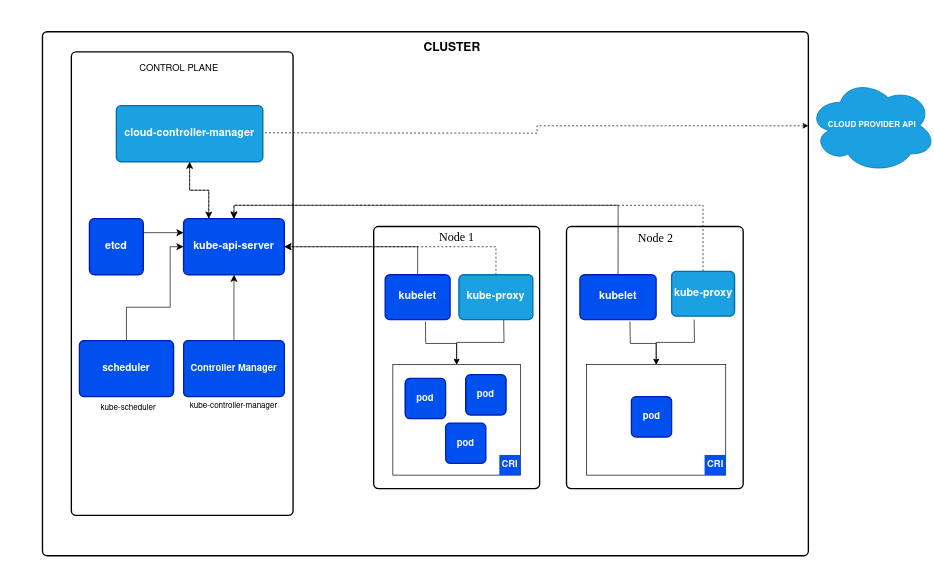
\includegraphics[width=450pt]{cluster-architecture.png}

Кластер Kubernetes состоит из набора рабочих машин, называемых узлами (Node), на которых выполняются контейнерные приложения \cite{k8s:cluster-architecture}. В каждом кластере есть хотя бы один рабочий узел.

На рабочих узлах размещаются поды (Pod), являющиеся компонентами рабочей нагрузки приложения. Плоскость управления (Control plane) управляет рабочими узлами и подами в кластере. В производственных средах плоскость управления обычно работает на нескольких компьютерах, а в кластере обычно работает несколько узлов, что обеспечивает отказоустойчивость и высокую доступность\cite{k8s:components}.

\subsection{Компоненты плоскости управления}
Компоненты плоскости управления принимают глобальные решения о кластере (например, планирование), а также обнаруживают события кластера и реагируют на них (например, запуск нового пода, когда их меньше, чем заданное администратором число)\cite{k8s:cp-components}.

Компоненты плоскости управления можно запускать на любой машине в кластере. Однако для простоты сценарии настройки обычно запускают все компоненты плоскости управления на одном компьютере и не запускают на этом компьютере пользовательские контейнеры.

\subsubsection{kube-apiserver}
Сервер API --- это компонент плоскости управления Kubernetes, который \\предоставляет интерфейс для плоскости управления Kubernetes. Основная реализация API-сервера Kubernetes --- kube-apiserver.

kube-apiserver предназначен для горизонтального масштабирования, то есть масштабируется за счет развертывания большего количества экземпляров. Возможно запустить несколько экземпляров kube-apiserver и балансировать трафик между ними.

\subsubsection{etcd}
etcd — это строго согласованное, распределенное хранилище значений ключей, которое обеспечивает надежный способ хранения данных, к которым должен иметь доступ кластер. В Kubernetes используется в качестве резервного хранилища для всех данных кластера.

\subsubsection{kube-scheduler}
Компонент плоскости управления, который отслеживает вновь созданные поды без назначенного узла и выбирает узел для их запуска.

Факторы, принимаемые во внимание при принятии решений по планированию, включают: индивидуальные и коллективные требования к ресурсам, ограничения аппаратного или программного обеспечения, политики, расположение днных, помехи между рабочими нагрузками и сроки.

\subsubsection{kube-controller-manager}
Компонент плоскости управления, который запускает процессы контроллеров, которые ответственны за управление отдельными компонентами кластера.

Существует много разных типов контроллеров. Некоторые примеры из них:
\begin{itemize}
   \item Контроллер узла: отвечает за обнаружение и реагирование при выходе узлов из строя.
   \item Контроллер заданий: отслеживает объекты заданий, которые представляют собой одноразовые задачи, а затем создает поды для выполнения этих задач до завершения.
\end{itemize}

\subsubsection{cloud-controller-manager}
Компонент плоскости управления Kubernetes, в который встроена логика \\управления, специфичная для облака. Диспетчер облачных контроллеров позволяет вам связать ваш кластер с API вашего облачного провайдера и отделить компоненты, которые взаимодействуют с этой облачной платформой, от компонентов, которые взаимодействуют только с вашим кластером.

Менеджер облачных контроллеров запускает только контроллеры, специфичные для вашего облачного провайдера. Если вы используете Kubernetes локально то в кластере нет менеджера облачного контроллера.

\subsection{Компоненты узла}
Компоненты узла запускаются на каждом узле, поддерживая работу подоылей и обеспечивая среду выполнения Kubernetes\cite{k8s:n-components}.

\subsubsection{kubelet}
Агент, работающий на каждом узле кластера. Он гарантирует, что контейнеры работают.

kubelet принимает набор спецификаций, предоставляемых с помощью различных механизмов, и гарантирует, что контейнеры, описанные в них, работают и исправны. kubelet не управляет контейнерами, которые не были созданы Kubernetes.

\subsubsection{kube-proxy}
kube-proxy --- это сетевой прокси, который работает на каждом узле вашего кластера.

kube-proxy поддерживает сетевые правила на узлах. Эти сетевые правила разрешают сетевое соединение с вашими подами из сетевых сеансов внутри или за пределами вашего кластера.

\subsubsection{Среда выполнения контейнеров}
Фундаментальный компонент, который позволяет Kubernetes эффективно \\запускать контейнеры. Он отвечает за управление выполнением и жизненным циклом контейнеров в среде Kubernetes.

Kubernetes поддерживает среды выполнения контейнеров, такие как containerd, CRI-O и любую другую реализацию Kubernetes CRI (интерфейс выполнения контейнера), например Docker.

\subsection{Сетевая модель}
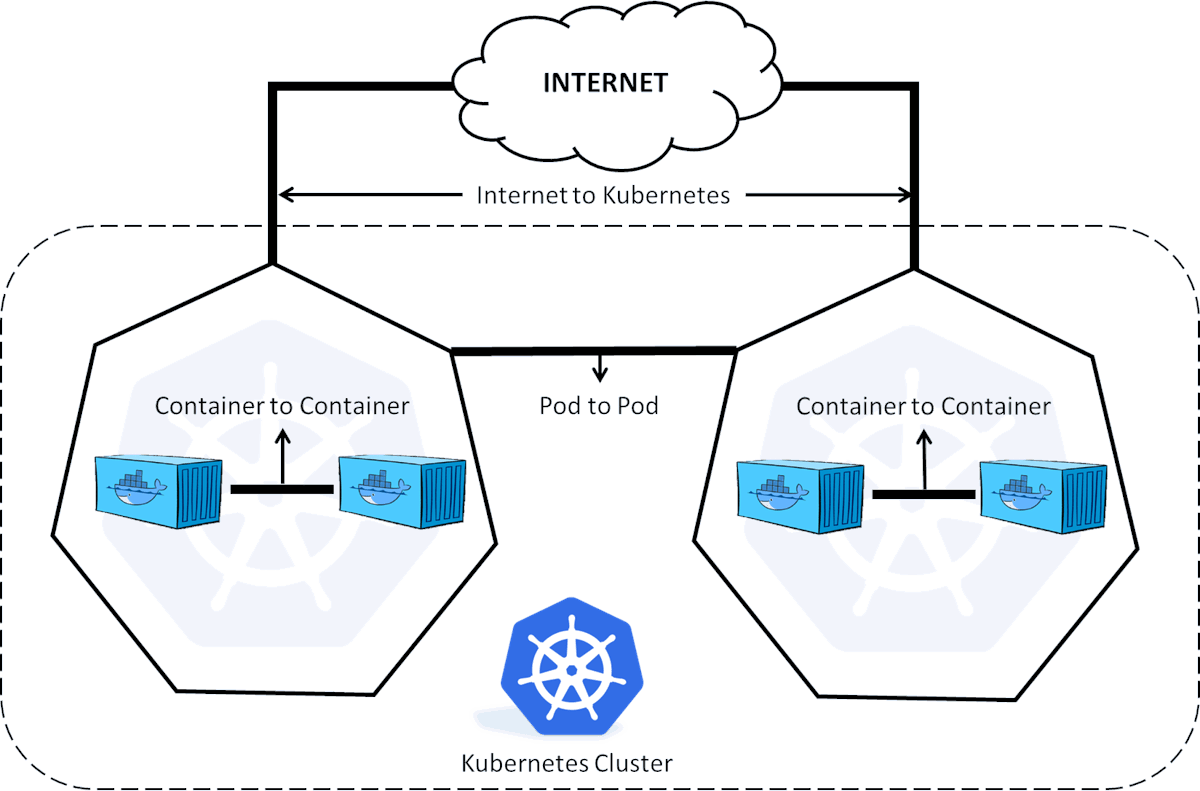
\includegraphics[width=450pt]{kubernetes-Networking-Model.png}

Каждый под в кластере получает свой собственный уникальный IP-адрес внутри всего кластера. Это означает, что не нужно явно создавать связи между подами, и вам почти никогда приходится иметь дело с сопоставлением портов контейнера с портами хоста\cite{k8s:network-model}.

Это создает чистую, обратно совместимую модель, в которой поды можно рассматривать как виртуальные машины или физические хосты с точки зрения распределения портов, именования, обнаружения служб, балансировки нагрузки, настройки приложений и миграции.

Kubernetes предъявляет следующие фундаментальные требования к любой сетевой реализации:
\begin{itemize}
  \item Поды могут взаимодействовать со всеми другими подами на любом другом узле без NAT.
  \item Агенты на узле (например, системные демоны или kubelet) могут \\взаимодействовать со всеми подами на этом узле.
\end{itemize}

Эта модель не только достаточно проста, но и совместима с желанием Kubernetes обеспечить легкий перенос приложений с виртуальных машин в контейнеры.

IP-адреса Kubernetes существуют в области пода --- контейнеры внутри пода совместно используют свои сетевые пространства имен, включая IP-адрес и MAC-адрес. Это означает, что все контейнеры одного внутри пода могут достигать друг друга как будто на локальном хосте. Это также означает, что контейнеры внутри пода должны координировать использование портов, но это ничем не отличается от процессов в виртуальной машине. Это называется моделью <<IP на каждый под>>.

Можно запросить порты на самом узле, которые пересылаются на под, но это очень узкоспециализированная операция. Сам под слеп к существованию или отсутствию таких портов.

Сеть Kubernetes решает четыре проблемы:
\begin{itemize}
   \item Контейнеры внутри пода используют для связи loopback.
   \item Сеть кластера обеспечивает связь между различными подами.
   \item Service API (API "Служба") позволяют сделать приложения, работающие в подах, доступным извне вашего кластера.
     \begin{itemize}
       \item Ingress предоставляет дополнительные функции, специально предназначенные для предоставления доступа к HTTP-приложениям, веб-сайтам и API.
     \end{itemize}
   \item Вы также можете использовать API Service для публикации служб только для использования внутри вашего кластера.
\end{itemize}

\subsection{Службы}
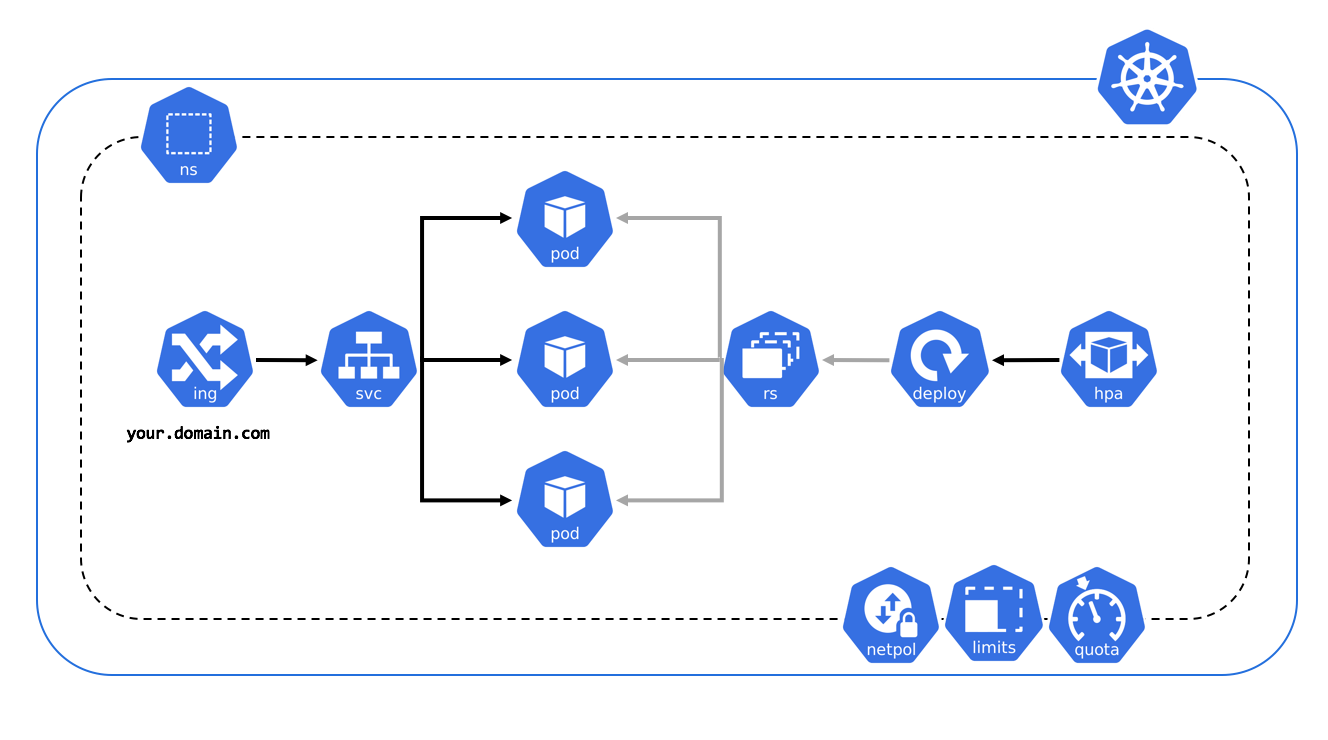
\includegraphics[width=450pt]{service.png}

В Kubernetes Service (служба, сервис) --- это метод предоставления доступа к сетевому приложению, которое работает как на одном, так и на нескольких подах\cite{k8s:service}.

Основная цель служб в Kubernetes --- убрать необходимости модифицировать существующее приложение для использования незнакомого механизма обнаружения сервисов. Вы можете запускать код в подах, будь то код, разработанный для облачного мира, или старое приложение, которое вы поместили в контейнер. Вы используете службу, чтобы сделать этот набор подов доступными в сети, чтобы клиенты могли с ним взаимодействовать.

Если вы используете спецификацию развертывания (Deployment) Kubernetes для запуска своего приложения, то оно может динамически создавать и уничтожать поды. Время от времени вы не знаете, сколько из этих подов работает и исправно; возможно, вы даже не знаете, как называются эти поды. Поды Kubernetes создаются и уничтожаются в соответствии с желаемым состоянием вашего кластера. Поды --- эфемерны. Не следует ожидать, что отдельный под будет надежным и долговечным.

API службы представляет собой абстракцию, помогающую предоставлять доступ к группам подов по сети. Каждый объект службы определяет логический набор конечных точек (обычно этими конечными точками являются поды), а также политику обеспечения доступа к ним.

Например, рассмотрим сервис обработки изображений, бакэнд которого запущен на трех подах. Эти поды взаимозаменяемы --- фронтэнду все равно, какой бакэнд он использует. Хотя фактические поды, составляющие бакэнд, могут меняться, фронтэнд об этом не знает, и он не отслеживает, где находится бакэнд. Фронтенд общается со службой, которая сама находит подходящий под бакэнда.

\subsection{Ingress}
\includegraphics[width=450pt]{enterprise-grade-IC-OpenShift_topology.png}

Если выши приложения используют HTTP, вы можете использовать Ingress для управления тем, как веб-трафик достигает этих приложений. Ingress не является службой, но он действует как точка входа в кластер. Ingress позволяет объединить правила маршрутизации в один ресурс, чтобы вы могли предоставлять единый доступ к нескольким компонентам приложений, работающим отдельно в разных подах.

Ingress может быть настроен для предоставления Сервисам URL-адресов, \\доступных извне, балансировки трафика, завершения SSL/TLS и предложения виртуального хостинга на основе имени\cite{k8s:ingress}. Контроллер Ingress отвечает за выполнение фонкций Ingress, обычно с помощью балансировщика нагрузки, хотя он также может настроить дополнительные интерфейсы для обработки трафика.

\newpage

\section{Список литературы}

% Print bibliography without heading
\printbibliography [heading=none]

\end{document}
